\subsection{Observed requests in real agent runs}
\label{sec:agent-observations}

\paragraph{Capture and scope.}
We reanalyzed eight SWE-bench Verified task runs~\cite{swebench2024}: five
Core and three Exploratory. All used DSH 0.1.5-rc.1 and the CCSwitch-configured
model \code{deepseek-v4-flash}. Exploratory runs used a broader
investigation/testing prompt and a 30-minute budget; all finished earlier.
Each base-commit checkout was mounted through \code{libfuse-fs}
\code{PassthroughFs} on Ubuntu 24.04 under WSL; \code{rfuse3}
\code{LoggingFileSystem} recorded actual FUSE handler requests.
Streaming reanalysis covered all 1,138,884 events: 217,129 Core and 921,755
Exploratory. Counts retain every status, 64 setup/canary requests before
agent startup, and teardown, including 24 requests after recorded run finish.
Group statistics weight requests equally, not tasks. Per-task counts and
source-validation details are in the companion workload record.

\begin{figure*}[!t]
\centering
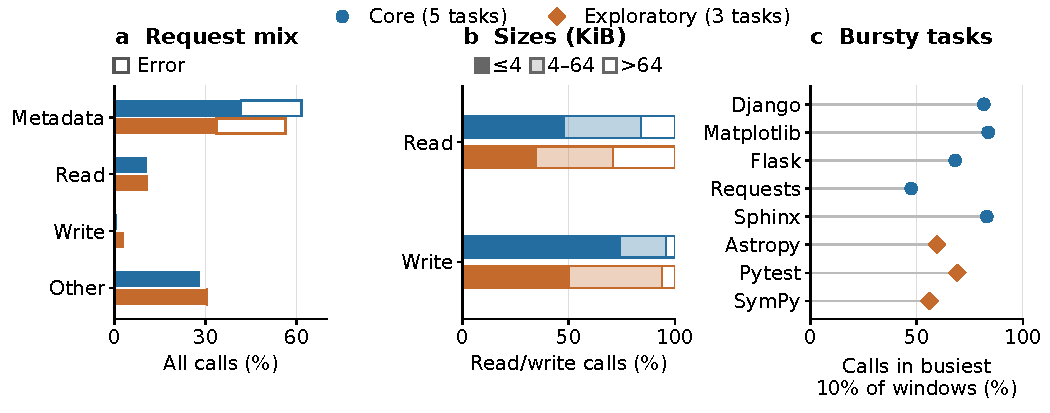
\includegraphics[width=\textwidth]{figures/agent-fuse/fuse-combined-compact.pdf}
\caption{Request structure across eight single-run FUSE captures.
Core bars precede Exploratory bars in each pair.
(a) Shares of all calls; white segments are errors within each total.
Metadata comprises \code{lookup}, \code{getattr}, \code{getxattr},
\code{readdirplus}, \code{opendir}, and \code{releasedir}; Other contains
every remaining method, including file open/flush/release.
(b) Each bar includes all reads or writes in its group. Dark, light, and white
segments denote $\leq4$, $(4,64]$, and $>64$ KiB, respectively
($1\,\mathrm{KiB}=1024$ bytes). Read counts are 22,142/98,292 and write
counts 1,112/23,600 (Core/Exploratory), all \code{ok}. Lengths are requested
FUSE bytes, not object sizes.
(c) Fraction of each task's calls in its busiest 10\% of one-second windows,
rounding the window count up; zero-call and final partial windows are retained.
All panels retain setup/teardown and every recorded status.}
\label{fig:agent-fuse-combined}
\end{figure*}

\paragraph{Metadata traffic and read dominance.}
The six metadata methods accounted for 61.5\% of Core and 56.4\%
of Exploratory calls (Figure~\ref{fig:agent-fuse-combined}a).
Restricting the denominator and numerator to \code{ok} events reduces these
shares to 52.0\% and 44.2\%: failed probes materially change the request mix.
Across tasks, the all-status share ranged from 39.6\% in SymPy to 65.4\% in
Django, so the group majority does not describe every task.
Read calls outnumbered writes by 19.9:1 in Core and 4.16:1 in Exploratory;
per-task ratios ranged from 3.12:1 (Pytest) to 42.7:1 (Matplotlib).
These observations motivate evaluating both positive and negative metadata
paths alongside data I/O.

\paragraph{A mixture of request sizes.}
Reads ranged from 4 to 128 KiB, with Core and Exploratory medians of 8 and
16 KiB. Writes ranged from one byte
to 128 KiB, with medians of 4,084 and 4,117 bytes, respectively.
Requests of at most 4 KiB accounted for 47.7\% and 34.5\% of reads, and
74.3\% and 49.9\% of writes. The interval $(4,64]$ KiB contained a further
36.2\% and 36.4\% of reads and 21.3\% and 44.0\% of writes
(Figure~\ref{fig:agent-fuse-combined}b).
This mixture motivates measuring how client fetching and uploads transform
requests before testing backend layouts. FUSE observations occur below kernel
caching and readahead; they do not identify application syscall sizes, unique
bytes, finalized object lengths, or an optimal block size.

\paragraph{Task and temporal heterogeneity.}
Tasks generated 8,542--634,726 calls. Astropy contributed 68.9\% of
Exploratory calls, versus 6.0\% for Pytest. Capture spans, from first to last
request start, were 42.7--71.3 seconds for Core and 119.9--556.1 seconds for
Exploratory. The busiest 10\% of one-second windows, rounded up per task,
contained 47.4--83.7\% of its calls (Figure~\ref{fig:agent-fuse-combined}c).
The companion record retains the full method breakdowns, size ECDFs,
and per-task cumulative time curves. Replay
should retain these per-task mixes and bursts. Each task was observed once;
different repositories, prompts, and budgets prevent a causal interpretation
of the group contrast. Without tool-phase labels, bursts cannot be assigned
to searching, editing, or testing.

\paragraph{Status semantics and evidence limits.}
The capture contained 872,519 \code{ok}, 253,669 \code{error}, and 12,696
\code{incomplete} events. Errors occurred in \code{lookup} (233,452),
\code{getxattr} (20,203), and \code{rmdir} (14). Collection notes associate
many with failed path probes or unsupported attributes; absent errno values
prevent event-level cause attribution. The parser labels a request
\code{incomplete} when no recognized completion is paired with it: here,
12,688 \code{forget} and eight \code{destroy} records. Neither label counts
failed agent tasks. All eight agent and daemon exit codes were zero, which
does not establish SWE-bench grading success.

Handler latency measures WSL passthrough intervals and excludes model response
time. Elapsed capture time instead includes inter-request gaps, which may
contain model waiting; summing overlapping handler intervals cannot recover
task wall time. These observations do not measure RustFS, Redis, network
object storage, or cloud-disk latency. They motivate metadata and mixed-I/O
experiments for this single-agent/model panel, but do not establish cross-task
sharing, sparse mutation, or performance gains from \sysname, RustFS, or
the automatic hint policy. Those remain questions for
Section~\ref{sec:evaluation}.
